3\chapter{Online Learning}\label{ch:OnlineLearning}
Online Learning is a theoretical framework to formalize a sequential decision problem in which an agent has to take consecutive actions in an environment. Every time the agent takes an action, the environment returns a loss signal (or reward depending on the convention on the sign). This framework is similar to other sequential decision problems such as Reinforcement Learning \cite{sutton1998introduction}, with the exception that the loss function is decided by an adversary which has complete knowledge of your strategy in advance, rather that be described by a stochastic probability kernel. \todo{Francesco dice che è sbagliato.}
The purpose of this section is to present the general framework of Online Game Playing and to introduce the notation necessary for the development of the theory. We will define formally the framework of Online Learning with Expert Advice, which is one the most studied framework of Online Learning, due to its ability to include many other frameworks, such as Multi Armed Bandit\todo{define} or Online Convex Optimization. \todo{maybe add DAgger}
Then we will present the concept of \emph{regret} and present the relationship of Online Learning to classical repeated games, a classical framework coming from the field of Game Theory. Modern finance \todo{manca coeasion OL->finance} has more and more the need for a Game Theoretic approach, this is evident when one looks at the field of on venue market making, that can be modeled naturally as a repeated game, or in merger and acquisition that can be modeled as a normal form game. \todo{add ref e aggiustare}
Finally we will introduce Online Convex Optimization as a special case of Online Learning with expert advice and its interesting relationship to theoretical statistical learning. The choice of this path, from Online Learning to Online Convex Optimization, has been done to show how general and powerful Online Learning is in its simplicity, and why Online Convex Optimization is the most suitable framework to present our contribution to Online Portfolio Selection, that will be presented in later chapters.\todo{ref  chapter ...}

In fact, even if we will focus on the portfolio problem, the apparently simple formulation of this framework is capable to encompass many other applications and problems, such as network routing~\cite{belmega2018online} and dark pool order allocation~\cite{agarwal2010optimal}. 
A thorough dissertation of the techniques that have been developed in the field of Online Learning can be found in \cite{cesa2006prediction}.
%Cita qualcuno he dia esposizione completa

\section{Online Learning}
\label{sec:OnlineLearning}
\begin{definition}(Online Game Playing).\label{def:OGP}
    Let $\mathcal Y$ be the outcome space, $\mathcal D$ the prediction space and $f:\mathcal D\times\mathcal Y\to \mathbb R$ is a loss function, an Online Game is the following sequential game played by the forecaster $\mathcal A$ and the environment:

    For each round $t\in 1,2,\ldots$
    \begin{enumerate}
        %\item Each expert $E_i\in\mathcal E$ choose its prediction $x_{t,E_i}\in\mathcal D$
        \item The learner $\mathcal A$ chooses an element of the decision space $x_t\in\mathcal D$.
        \item The environment chooses the element $y_t\in\mathcal Y$, and subsequently determines the loss function $f(\cdot,y_t)$.
        \item The agent $\mathcal A$ incurs in a loss $f(x_t,y_t)$.
		\item The agent updates its cumulative losses $L_t=L_{t-1}+f(x_t,y_t)$ with $L_0=0$
    \end{enumerate}
\end{definition}

In Online Learning an agent $\mathcal A$ has to guess the outcome $y_t$ based on a the past outcomes $y_1,y_2,\ldots,y_{t-1}$ of some events that are in the outcome space $\mathcal Y$, at each time step she will play (sometimes we will also say \emph{predict}) $x_t$, that is an element of the prediction space $\mathcal D$, and the environment will choose a loss function $f(\cdot,y_t)$ by determining the outcome $y_t$.
Sometimes it is not important to know the exact outcome of the round and so we can identify the function $f(x,y_t)$ with $f_t(x)$. The agent $\mathcal A$ is essentially the identification of the functions that maps the history of past outcomes to the new prediction:
$$\mathcal A\equiv\left\{h_{t-1}:=(y_1,\ldots,y_{t-1})\longmapsto x_t\right\}_{t\ge 1} $$
The simplest case is for $\mathcal Y=\mathcal D$ and both of finite cardinality, meaning that there are only a finite number of actions that the agent $\mathcal A$ can choose from. 
We will sometimes refer to the environment defined in Section \ref{def:OGP} as "adversarial", since no stochastic characterization is given to the outcome sequence $y_t$ and the analysis of the regret is done assuming a worst case scenario.
Since the adversary knows the prediction $x_t$, before deciding the outcome $y_t$, absolute minimization \todo{???} of the loss is an hopeless task and so we have to set an easier task. We will also present the counterexample to why the absolute minimization of the loss is an hopeless task, and present the adapt minimal framework to successful Online Learning in Adversarial Environment.

% ==================================================

% The assumption\todo{Non qui} of a model for the data even existing is basically assuming the stationarity of the observed events. This may be reasonable in some cases, like speech recognition in which we can assume that there is constant model which translate sound of speech into its lexical transliteration, but it not as reasonable in other cases, as trivial as spam filtering. In email classification for spam filtering, the spam writers actually adapts to the filter itself and every constant model would eventually be out of fashion after some time. In such a regime you need a way of adapting your hypotheses during the learning procedure. This is were Online Learning comes to help. In Online Learning we do not make any assumption on the structure of the data and constantly adapting our hypothesis in order to asymptotically perform as the best hypothesis in hindsight.

% =================================================

\subsection{Regret and Experts}
\begin{figure}[t!]
\centering
\begin{pspicture}(0,-3.42)(8.18,3.42)
\psframe[linecolor=black, linewidth=0.04, dimen=outer, framearc=0.1](6.54,0.9)(2.78,-0.36)
\psframe[linecolor=black, linewidth=0.04, dimen=outer, framearc=0.1](6.52,3.42)(2.82,2.3)
\rput[bl](3.76,2.7){Agent: $\mathcal A$}
\rput[bl](3.68,0.12){Environment}
\psline[linecolor=black, linewidth=0.036, arrowsize=0.05291667cm 2.0,arrowlength=1.4,arrowinset=0.0]{->}(6.54,2.8)(7.66,2.8)(7.66,0.2)(6.54,0.22)
\rput[bl](7.9,1.44){$x_t$}
\psline[linecolor=black, linewidth=0.036, arrowsize=0.05291667cm 2.0,arrowlength=1.4,arrowinset=0.0]{->}(2.78,0.3)(1.46,0.3)(1.46,2.88)(2.8267796,2.8677726)
\rput[bl](0.0,1.2){$f(x_t,y_t)$}
\psframe[linecolor=black, linewidth=0.036, dimen=outer, framearc=0.1](6.2,-2.2)(3.16,-3.42)
\rput[bl](3.78,-2.92){Experts: $\mathcal E$}
\rput[bl](2.96,-1.36){$x_{e,t}$}
\rput[bl](5.26,-1.34){$f(x_{e,t},y_t)$}
\psline[linecolor=black, linewidth=0.036, arrowsize=0.05291667cm 2.0,arrowlength=1.4,arrowinset=0.0]{->}(3.8,-2.22)(3.8,-0.36)
\psline[linecolor=black, linewidth=0.036, arrowsize=0.05291667cm 2.0,arrowlength=1.4,arrowinset=0.0]{->}(5.18,-0.4)(5.18,-2.22)
\end{pspicture}

\caption{Online Learning with Expert Advice as Multi Agent-Environment interaction.}
\label{fig:OL}
\end{figure}
We stated that the objective of absolute loss minimization is hopeless in an adversarial framework, as the adversary can always choose the outcome $y_t$ that maximizes the loss $f(x,y_t)$ regardless of the decision $x\in\mathcal D$ taken by the learner. We shall present a simple counterexample in this setting.

Take $\mathcal D$ as a space of binary outcomes, \emph{i.e.} $|\mathcal D|=2$ absolute loss as $f(x,y)=|x - y|$. Since the adversary plays after the learner $\mathcal A$, it can  make the loss of the learner $L_T=T$ by outputting the bit non predicted by the learner. Notice that no assumption has been made on the strategy followed by the learner $\mathcal A$.
From this example it is clear that the learner has to set a less ambitious goal.

We do so by extending the theoretical formulation in Section \ref{sec:OnlineLearning} by including a set $\mathcal E$ of other players, this setting is called "prediction with expert advice". At each time step of the prediction game, each expert $e\in\mathcal E$, predicts an element $x_{t,e}\in\mathcal D$, and incurs in a loss $f(x_{t,e},y_t)$, just as the agent $\mathcal A$, creating a general multi-agent interaction as in Figure~\ref{fig:OL}. \todo{Spiegare figure: Non l'ho già fatto?}
Now the goal that the learner sets itself to solve is to obtain small losses with respect to the best expert in the class $\mathcal E$. This concept is captured by the definition of regret.
Formally, we define the regret $R_{T,e}$ for the agent $\mathcal A$ with respect to expert $e\in\mathcal E$ (assumed finite for the moment) as follows:

\begin{equation}\label{def:Regret}
	R_{T,e} = L_T-L_{T,e}
\end{equation}

The regret observed by the agent $\mathcal A$ with respect to the entire class of experts $\mathcal E$ is defined as:

\begin{equation}
	R_T=\max\limits_{e\in\mathcal E}R_{T,e}=L_T-\min\limits_{e\in\mathcal E}L_{T,e}.
\end{equation}

The task the agent $\mathcal A$ is set to solve is to find a sequence $x_t$ function of the information obtained up to the time $t$ in order to obtain small regret $y_T$ with respect to any sequence $y_1,y_2,\ldots$ chose by the environment.

In particular we aim to achieve sub-linear regret $y_T= o(T)$, meaning that the per-round regret $y_T/T$ will asymptotically vanish: 

\begin{equation}
	y_T= o(T) \implies \lim\limits_{T\to \infty}\frac{y_T}{T}=0,
\end{equation}

where $ o(T)$ is the space of sub-linear affine functions. A strategy $\mathcal A$ that attains sub-linear regret is called \emph{Hannan-Consistent}~\cite{hannan1957approximation}.

The regret is a measure of the distance between our online performance and the best offline (in retrospect) performance among the expert class $\mathcal E$, this is also called \emph{external regret} since it is compared to the external set of experts $\mathcal E$. A surprising fact is even that such algorithms do even exist.
Indeed a first result is that in general there are no Hannan Consistent strategies, and just introducing the concept of regret is not enough for successful Online Learning: 

A first simple counterexample can be found in~\cite{cover1966behavior}. If the decision space $\mathcal D$ is finite then there exists a sequence of loss function such that $R_T=\Omega(T)$.
% Cover Impossibility
Again take $\mathcal D$ as a space of binary outcomes, absolute loss as $f(x,y)=|x - y|$, and the class of experts is composed by two experts, one predicting always $0$ and the other always $1$. Taking $T$ odd, we have that the loss of the best expert is $L_{T,e}<\frac{T}{2}$, and we have already shown that the adversary can make the loss of the learner $L_T=T$. It is now evident that the regret is $R_T>T-\frac{T}{2}$, which do not allow $R_T/T\to 0$. This argument is easily extended in the case of any finite decision space $\mathcal D$.

In order for the learner to achieve sub-linear regret is to randomize its predictions, the learner, at each turn $t$, holds a probability distribution on the decision space and plays $x_t$ according to this distribution. Clearly the adversary has knowledge of the probability distribution of the learner $\mathcal A$, but has no knowledge of the random seed used by the agent $\mathcal A$, \emph{i.e.} does not know the actual decision taken according to the distribution held by the agent. If the original decision space was $\mathcal D$ with $|\mathcal D|=N$ after the randomization of the decision, we effectively transformed the decision space $\mathcal D$ into the $\Delta_{N-1}\in\mathbb R^{N}$ probability simplex. By doing so we are formally extending the game into its mixed extension, as will be discussed further in Section \ref{sec:GT}. It can be viewed also as a \emph{covexification} of the domain, pointing to the undeniably necessity of convex geometry in this context, that will be discussed in \ref{sec:OCO}. Therefore, from now on the domain $\mathcal D$ will be convex, either by the problem specification or by randomized convexification if the problem has discrete decision space.

\subsection{Existence of No-Regret Strategies}
In this section we will show the existence of Hannan-consistent strategies in the case of finite experts and provide a general form to generate sub-linear regret strategies. 
The general idea with a finite class of experts is given by the Weighted Average Forecaster. A natural class of algorithm to explore is the predicting as the weighted average prediction of the experts predictions, weighted on the accrued regret suffered by the agent $\mathcal A$:

\begin{definition}(Weighted Average Forecaster).\label{def:weighted_avg}
For a finite class of experts $\mathcal E$ the weighted average prediction is defined as
\begin{equation}
	x_t = \frac{\sum\limits_{i=1}^{N}w_{t-1,i}x_{t,i}}{\sum\limits_{i=1}^{N}w_{t-1,i}},
\end{equation}
where $w_{t-1,i}>0$ and $x_{t,i}$ is the prediction of expert $E_i\in\mathcal E$ at round $t$. 
\end{definition}

Since $\mathcal D$ is convex we have that $x_t\in\mathcal D$.
Then it is natural to assume that the weights are a function of the cumulated regret suffered by the agent with respect to the experts, and also that the change in weight is proportional to the change in a potential function:
We can generalize the simple weighted average prediction \eqref{def:weighted_avg} in the following general form, introduced in~\cite{cesa2003potential}:

\begin{equation}\label{eq:potential_avg}
x_t = \frac{\sum\limits_{i=1}^{N}\partial_i \Phi(\mathbf R_{t-1}) x_{t,i}}{\sum\limits_{i=1}^{N}\partial_i \Phi(\mathbf R_{t-1}) },
\end{equation}

where $\Phi(\mathbf u)=\varphi\left(\sum\limits_{i=1}^N\phi(u_i)\right)$ is a function $\Phi:\mathbb R^N\to\mathbb R^+$ defined through two increasing functions $\phi,\varphi:\mathbb R\to\mathbb R^+$, $\varphi,\phi\in\mathcal C^2(\mathbb R)$ and concave and convex, respectively and $\mathbf R_T=(R_{T,1},\ldots,R_{T,N})$.
By specializing the two functions $\varphi,\phi$ we can derive most of the algorithm for dealing with prediction under expert advice.
The reasons behind the general form of Equation \eqref{eq:potential_avg} and an extended discussion can be found in~\cite{hart2001general},~\cite{cesa2003potential} and~\cite{blackwell1956analog}, but the general idea is that the form of Equation \eqref{eq:potential_avg} has the following property:

\begin{theorem}
	If $x_t$ is given by Equation~\eqref{eq:potential_avg} and the loss $f(\cdot,y)$ is convex in the first argument then the instantaneous weighted regret satisfies:  
	$$\sup\limits_{y_t\in\mathcal Y}\sum\limits_{i=1}^N[f(x_t,y_t)-f(x_{t,i},y_t)]\partial_i \Phi(\mathbf y_{t-1}) \le 0$$.
\end{theorem}

\begin{proof}
	By convexity of $f(\cdot,y_t)$ we have that 
\begin{align}
	f(x_t,y_t)\le\frac{\sum\limits_{i=1}^N\partial_i\Phi(\mathbf R_{t-1})f(x_{t,i},R_t)}{\sum\limits_{i=1}^N\partial_i\Phi(\mathbf R_{t-1})}, \forall y_t\in\mathcal Y\label{eq:blw_cond}
\end{align}
And since $\Phi(\mathbf x)=\varphi\left(\sum\limits_{i=1}^N \phi(x_i)\right)$ we have that $$\partial_i\Phi(\mathbf x)=\varphi'\left(\sum\limits_{i=1}^N\phi(x_i)\right)\phi'(x_i)\ge0$$
Hence we can rearrange the terms in Equation~\eqref{eq:blw_cond} to obtain the statement.
\end{proof}

Note that fixing the structure for the weights as in Equation \eqref{eq:potential_avg} we have that $w_{t,i}\propto\phi'(R_{t,i})$ that is an increasing function in $R_{t,i}$ (since $\phi$ is convex and increasing) that essentially states that we are increasing the probability of playing actions on which we saw high regret $R_{t,i}$\todo{check}.

\begin{definition}\label{eq:ewf}
	The exponentially weighted algorithm is \eqref{eq:potential_avg} with $\varphi(x)=\frac{1}{\eta}ln(x)$ and $\phi(x)=e^{\eta x}$ giving weights of the form $w_{t-1,i}=e^{\eta y_{t-1,i}}/\sum\limits_{j=1}^Ne^{\eta y_{t-1,j}}$
\end{definition}

It can be shown \todo{e allora show} that the algorithm defined by the update rule in Equation \eqref{eq:ewf}, and for a convex loss function $f(\cdot,y_y)$, gives the following guarantee on the regret:
\begin{equation}\label{eq:regret_ewf}
R_T\le \frac{log(N)}{\eta}+\frac{T\eta}{8}\end{equation},

By choosing $\eta=O\left(\sqrt\frac{1}{T}\right)$ we obtain a sub-linear regret $R_T=\mathcal O(\sqrt T)$. %It is also possible to make this algorithm an all-time algorithm (no need to know the length of the game $T$, as opposed as a \emph{one-time} algorithm) by using the so called doubling trick by continually adapting the parameter $\eta$. In general a one-time algorithm obtains slightly smaller bounds then the all-time counterparts, that require the knowledge



\subsection{Experts}
The theoretical framework described in Section \ref{sec:OnlineLearning} is very general and most suited for a game theory analysis of the problem. This help us describe many other frameworks, such as Online Optimization, or Multi Armed Bandit (MAB) as embedded into a Game Playing framework with expert advice. It can then be specialized by fixing many elements of the definition, in order to be applied to the specific problem we are willing to solve.
For instance, the class of experts $\mathcal E$ is most of the time completely fictitious, meaning that the experts are not real players of the game, but most of the time they are \emph{simulable} meaning that the agent $\mathcal A$ is able to compute $x_{t,e}$ for each expert $e\in\mathcal E$ and most of the times the class of expert is very limited in its actions, \emph{e.g.} $\mathcal E$ is the class of experts for which $x_{t,e}$ is constant in $t$. In this case, which is the most studied class of experts, we are basically just comparing our learner $\mathcal A$ to the best fixed action $x^*$ in hindsight. This is a clairvoyant strategy that attains the minimum cumulative loss over the entire length of the game $T$.

\subsection{Uncountable Experts}\label{sec:uncountable_exp}

In the case of uncountable experts the Exponentially Averaged Prediction cannot be applied directly, but can be extended to a continuous mixture of experts predictions. More specifically we need the case of the class $\mathcal E$ being generated by a convex hull of a finite number of a base class of experts, $\mathcal E_N$.
With continuous class of experts $\mathcal E$ defined in this way, the regret definition becomes:

\begin{equation}
    R_T = \sup\limits_{q\in\Delta_{N-1}}R_{T,q}:=L_T-\inf\limits_{q\in\Delta_{N-1}}L_{T,q},
\end{equation}



where $\Delta_{N-1}\subset \mathbb R^{N}$ is the $N$-simplex, and 

$$L_{T,q}=\sum\limits_{t=1}^T f(\langle q,x_{t,e}\rangle,y_t),$$
where $x_{t,e}=(x_{t,1},\ldots,x_{t,N})\in\mathbb R^N$ is the vector of expert predictions at time $t$.
\subsection{Exp-Concave loss functions}
It will be important for the study of Portfolio Optimization the exp-concave class of loss functions.
$f(\cdot,y)$ is $\nu$-exp concave if $e^{-\nu f(\cdot,y)}$ is concave.

\begin{theorem}\label{th:General_Blk}
The Exponentially Weighted Average forecaster, for $\nu$-exp concave loss functions and for $\eta=\nu$ has the following property:

$$\Phi(\mathbf R_T)\le \Phi(\mathbf R_0)$$

where $\Phi(x)=\varphi\left(\sum\limits_{i=1}^N\phi(x_i)\right)$ is chosen as $\varphi(x)=\frac{1}{\nu}log(x)$ and $\phi(x)=e^{\nu x}$

\end{theorem}

\begin{proof}
    The weights are given by $w_{t-1,i}=e^{\nu y_{t-1,i}}/\sum\limits_{j=1}^N e^{\nu y_{t-1,j}}$.
    By exp-concavity we have that
    \begin{equation}
        e^{-\nu f(x_t,y_t)}=exp\left\{-\nu f \left(\frac{\sum\limits_{i=1}^N w_{t-1,i}x_{t,i}}{\sum\limits_{i=1}^N w_{t-1,i}},y_t\right)\right\}\ge \frac{\sum\limits_{i=1}^N w_{t-1,i}e^{-\nu f(x_{t,i},y_t)}}{\sum\limits_{i=1}^N w_{t-1,i}}
    \end{equation}
    this can be rewritten as 
    \begin{equation}\label{eq:conc_exp_last}
        \sum\limits_{i=1}^N e^{\nu y_{t-1,i}}e^{\nu [f(x_t,y_t)-f(x_{t,i},y_t)]}\le \sum\limits_{i=1}^N e^{\nu y_{t-1,i}}
    \end{equation}
    Applying $\varphi(x)=\frac{1}{\nu}log(x)$ to both sides of equation \eqref{eq:conc_exp_last} we obtain that $$\Phi(\mathbf R_{t})\le \Phi(\mathbf R_{t-1})$$ that prove the thesis.
\end{proof}

The case of exp concave functions is very special, since we can obtain Theorem~\ref{th:General_Blk} that can be used to prove regret bounds very easily:

\begin{equation}\label{eq:regret_exp_finite}
    R_T\le \frac{1}{\eta}\log\left(\sum\limits_{i=1}^N e^{\nu R_T,j}\right)=\Phi(\mathbf R_T)\le\Phi(\mathbf R_0) = \frac{log N}{\eta}
\end{equation}

The case of exp-concave losses is also useful for the case of uncountable experts sketched in Section~\ref{sec:uncountable_exp}. This formulation will be of central importance for the portfolio optimization problem.

It is natural to extend the Exponential Weighted Majority algorithm described by equation \eqref{def:weighted_avg} into its continuous case by:

\begin{equation}\label{eq:mixture}
    x_t=\frac{\int\limits_{\Delta_{N-1}} w_{q,t-1}\langle q,x_{t,e}\rangle dq}{\int\limits_{\Delta_{N-1}} w_{q,t-1}dq}
\end{equation}

\begin{theorem}(Mixture forecaster for exp-concave losses).\label{th:mixture_forecaster}
    Choosing $w_{q,t-1}=exp\left\{-\eta\sum\limits_{s=1}^{t-1}f(\langle q,x_{t,e}\rangle,y_s)\right\}$ in Equation \eqref{eq:mixture}, for a bounded $\nu$-exp concave loss function $f(\cdot,y)$, we obtain
    $$R_T\le N\nu\left(log\left(\frac{\nu T}{N}\right)+1\right)$$
\end{theorem}

Even in the case of uncountable many experts, exp-concavity of the loss function gives a better convergence rate of $\mathcal O(\log T)$then the exponentially weighted algorithm in Equation~\eqref{eq:regret_ewf}, which is $\mathcal O(\sqrt T)$.

% REGRET MINIMIZATION IN GAMES =================================================
\section{Regret Minimization in Games}
\label{sec:GT}\todo{Forse da togliere tutto questo s{}ubchpt}
In this section we explore the connection of the framework of Section \ref{sec:OnlineLearning} into a more classical repeated game framework. In the previous Section we looked at the adversary as a black box, without any specific model in mind. The reason of this chapter is to clarify its role as a player in the game and to show the game theoretical properties of Hannan-consistent agents. Since in Online Learning the convention is to speak about losses, we shall speak about losses (minimization) also in the classical definitions of game theory instead of payoffs (maximization).

\begin{definition}(Strategic Form $K$-Player Game).\label{def:Game}
    A Strategic form $K$-player game is t a tuple $\langle\mathcal K,\{X_i\}_{i\in\mathcal K},\{l_i\}_{i\in\mathcal K}\rangle$ where
    \begin{enumerate}
        \item $\mathcal K=\{1,\ldots,K\}$ is the finite set of players
        \item $X_i$ is the set of actions available to player $i\in\mathcal K$
        \item $l_i:\bigotimes\limits_{k=1}^KX_i\to\mathbb R$ is the loss observed by player $i\in\mathcal K$
    \end{enumerate}
	The game is called finite if $|X_i|<+\infty$ for all $i\in\mathcal K$.
\end{definition}


\subsection{Mixed extension}\label{sec:mixed}
As in Section~\ref{sec:OnlineLearning} we saw that it is impossible to obtains sub-linear regret in adversarial environment with finite decision space $\mathcal D$. A first step to solve this has been the \emph{randomized convexification}, where finite action spaces are extended into convex sets, given by their probability simplex, also losses are to be interpreted as expected losses when the mixed extension is applied to the formal game. More formally: 

\begin{definition}(Mixed-extension for finite games).
A finite game $\langle\mathcal K,\{X_i\}_{i\in\mathcal K},\{l_i\}_{i\in\mathcal K}\rangle$ can be extended into the game $\langle\mathcal K,\{\tilde X_i\}_{i\in\mathcal K},\{\tilde l_i\}_{i\in\mathcal K}\rangle$
\begin{enumerate}
	\item $\tilde X_i=\Delta_{|X_i|-1}\subset \mathbb R^{|X_i|}$ for all $i\in\mathcal K$ 
	\item $\tilde l:\bigotimes \tilde X_i\to\mathbb R$ is defined as
	$$\tilde l(x_1,\ldots,x_K)=\sum\limits_{i_1=1}^N\cdots\sum\limits_{i_K=1}^Np_{i_1}\ldots p_{i_K}l(i_1,\ldots,i_K)$$ 
\end{enumerate}
\end{definition}

Due to the impossibility result of Cover~\cite{cover1966behavior}, we have to work with the mixed extension formulation of the game. So from now on we take this step implicitly.
The taxonomy of game definition is quite extended and complex, we will focus on non-cooperative games \todo{cita qualcuno} since they are closely related to the setting tacked in the Online Learing field. More specifically, we will need the model for \emph{Zero Sum Game}. 

\begin{definition}($2$-Player Zero-Sum Game).\label{def:ZSG}
A Zero Sum game is a tuple $\langle\{X_1,X_2\},l:X_1\times X_2\to\mathbb R\rangle$. As in Definition~\ref{def:Game} $X_1,X_2$ are the action spaces for Player $1$ (row player) and Player 2 (columns player) respectively and $l(x_1,x_2)$ for $x_i,x_2\in X_1\times X_2$, represents the losses for Player $1$ and profits for player $2$.
\end{definition}

If this game is played for $T$ turns, we can call it a repeated game, and the losses for each player will be $L_1^{(T)}=\sum\limits_{t=1}^Tl_i\left(x_i^{(t)},x_2^{(t)}\right)$ and $L_2^{(T)}=-L_1^{(T)}$. 


\subsection{MinMax Consistency}
The question of what guarantees does Hannan-consistent strategies bring to the game theoretical formulation of the problem, and why Online Learning is sometimes called \emph{Learning in Games}.
For such games we can define a \emph{values} for the game as: 
\begin{align}
    V_1=\inf\limits_{x_1\in X_1}\sup\limits_{x_2\in X_2}l(x_1,x_2)\\
	V_2=\sup\limits_{x_2\in X_2}\inf\limits_{x_1\in X_1}l(x_1,x_2)
\end{align}

These is the value that the players can guarantees themselves, meaning that no matter the strategy of the columns player, the row player could guarantee himself a loss of at maximum $V_1$, the converse holds for the row player. It can be interpreted as the minimum loss (best payoff) that player could achieve if we know that the other player would play adversarially. It is clear that $V_2\le V_1$. In the case the zero sum-game is a mixed extension of a finite game, then the Von Neumann theorem states that $V_1=V_2$.
 
Now we will embed the framework of Online Game Playing of Section \ref{sec:OnlineLearning} in a two player zero sum game. 
Online Learning is a special form of Zero Sum Game (possibly considering its mixed extension described in Definition \ref{sec:mixed}) where $X_1\equiv \mathcal D$ and $X_2\equiv \mathcal Y$. The loss function $l:X_1\times X_2\to\mathbb R$ can be identified by the loss $f:\mathcal D\times \mathcal Y\to\mathbb R$ of the Online Learning Agent $\mathcal A$.
Now we will explore interesting properties of Hannan Consistent strategies. A surprising fact is that if the row player plays accordingly to a Hannan Consistent strategy then it achieve the value of the game $V_1$. 

\begin{theorem}
    Hannan Consistent agents in Online Game Playing reach asymptotically the minmax value of the one shot game.
    $$\limsup\limits_{T\to +\infty}\frac{1}{T}\sum\limits_{t=1}^Tf(x_t,y_t)\le V_1$$
\end{theorem}

\begin{proof}
    Let us suppose that player $1$ plays an Hannan Consisten strategy and that $y_1,y_2,\ldots \subset \mathcal Y$ is a generic sequence played by the columns player.
    \begin{equation}
        \limsup\limits_{T\to+\infty}\frac{y_T}{T}\le0
    \end{equation}
    
    that can be translate into 
    \begin{equation}\label{eq:second_HC}
        \limsup\limits_{T\to+\infty}\frac{1}{T}\sum\limits_{t=1}^Tf(x_t,y_t)\le\limsup\limits_{T\to+\infty}\frac{1}{T}\inf\limits_{x\in\mathcal D}\sum\limits_{t=1}^Tf(x,y_t)
    \end{equation}

    Lets call $\hat y_T$ the empirical distribution played by player $2$ up to $T$:
    $$\hat y_T(j)=\frac{1}{T}\sum\limits_{t=1}^Ty_t$$
    by \eqref{eq:second_HC} we just need to show $\frac{1}{T}\inf\limits_{x\in \mathcal D} \sum\limits_{t=1}^T f(x,y_t)\le V$

    \begin{align}
        \inf\limits_{x\in\mathcal D}\frac{1}{T}\sum\limits_{t=1}^T f(x,y_t)=\inf\limits_{x\in\mathcal D} f(x,y_T)\le\sup\limits_{y\in\mathcal Y}\inf\limits_{x\in\mathcal D} f(x,y)\le V_1
    \end{align}
\end{proof}

We showed that regardless of the strategy of player $2$, a player playing a Hannan Consistent strategy achieves lower losses that the value of the game $V_1$. Clearly using a Hannan consistent strategy means that if player $2$ were not adversarial, then player $1$ could potentially earn a significantly higher average payoff than the value $V$ of the game. By symmetry if both players play an Hannan Consistent strategy than they will asymptotically reach the value of the game $V=V_1=V_2$.

\begin{figure}[t!]
    \centering
    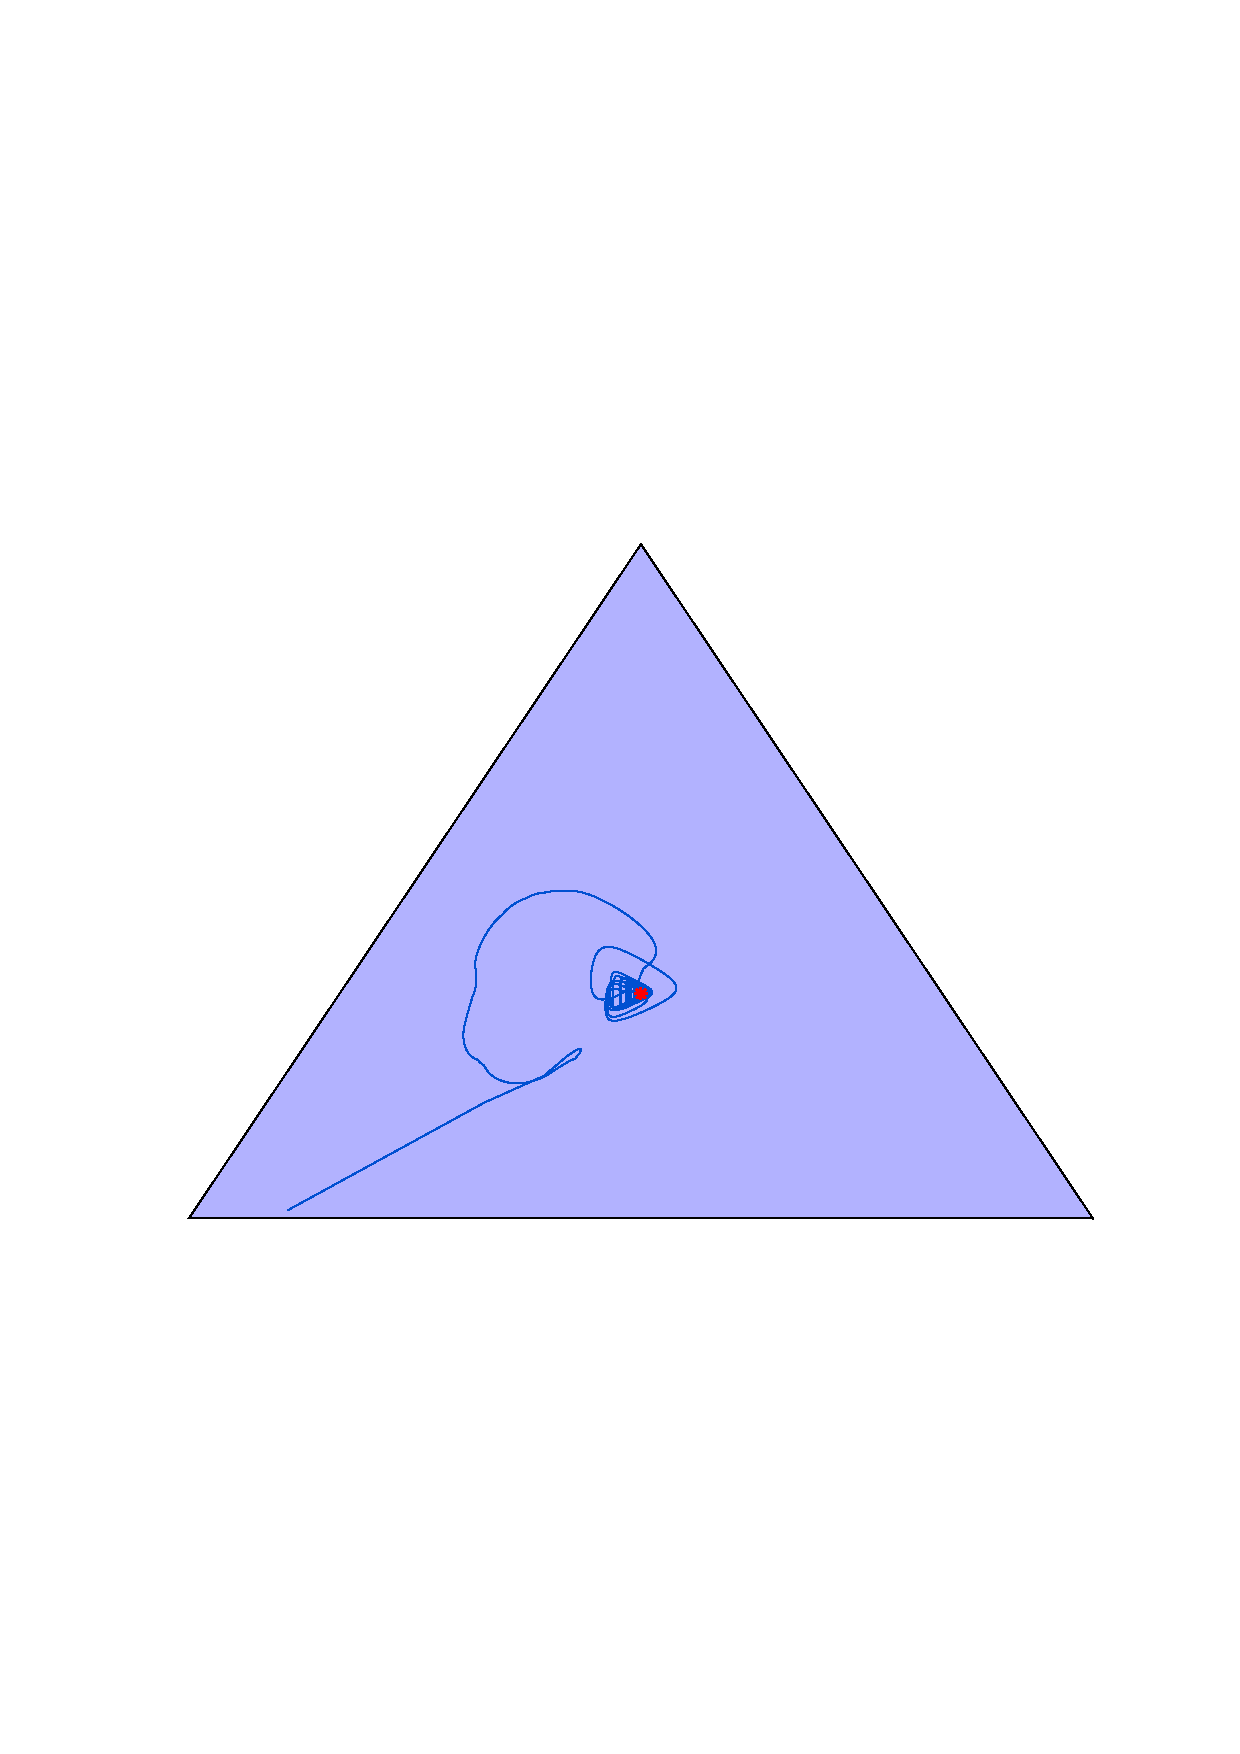
\includegraphics[width=8cm]{./img/rps_ewm.pdf}
\caption{Rock Paper Scissor Dynamics Exponentially Weighted Majority}
\label{fig:RPS}
\end{figure}

\section{Online Convex Optimization for Regret Minimization}\label{sec:OCO}

Let's compare this framework to an apparently unrelated problem, namely optimization, this will be the most suited framework to embed the Online Portfolio Optimization Problem. In online optimization an agent $\mathcal A$ is set to optimize a sequence of functions $f_t(x)$ where usually $f_t:\mathcal X\to \mathbb R$ is a real valued function from the set $\mathcal X\subset\mathbb R^n$. IN Online Convex Optimization literature, some times the loss functions are identified as $f(x,y_t)\equiv f_t(x)$.
The decision space $\mathcal D$ is assumed to be convex, as the are the functions $f_t:\mathcal D\to \mathbb R$. This framework was first devised in \cite{zinkevich2003online}, and has been later wildly used in the machine learning community to engineer optimization procedures \cite{shalev2012online}. 

Convexity plays an central role in most of the analysis made in Online Learning, and Online Convex Optimization. Convexity of the domain $\mathcal D$ and of the loss functions, $f(\cdot,r)$ bound the problem geometry and let us derive simple and efficient learning procedures. More generally in the subsequent section we will present the general learning.

\subsection{A General Algorithm for Online Convex Optimization}

In this Section we will see an algorithm called \emph{Online Mirror Descent} (OMD), that generalizes many Online Convex Optimization algorithms. It is a first order method that works in the dual space defined by the choice of some regularizator \todo{regularizator?}. The OMD algorithm is genral and optimal in the sense that every Online Convex problem can be learned online nearly optimally with OMD, the precise formulation can be found in \cite{srebro2011universality}.

OMD works with a class of regularitators called Bregman Divergences, \cite{banerjee2005clustering}.

\begin{definition}(Bregman divergence). Given a differentiable convex function $\psi:\mathcal X\to\mathbb R$ the Bregman divergence is defined as an operator $d_{\psi}:\mathcal X\times\mathcal X\to \mathbb R^+$ defined for $x,y\in\mathcal X\times\mathcal X$ as 
\begin{equation}\label{eq:bregman_div}
d_\psi(x,y)=\psi(x)-\psi(y)-\langle x-y,\nabla \psi(y)\rangle
\end{equation}
\end{definition}

Since $\psi$ is convex we have that $d_\psi(x,y)\ge0$, we can see that by linearization of $\psi(x)$ around $y\in\mathcal X$ and by the inequality on the non standard inner product defined by the hessian of the function $\psi$ which is positive thanks to the convexity. Since the operator defined in Equation \eqref{eq:bregman_div} is not symmetric in its arguments, it does not define an metric in the space $\mathcal X$.

For $\psi(x)=||x||_2^2$ then $d_\psi(x,y)=||x-y||_2^2$. For $\psi(x)=\sum\limits_{i=1}^Nx_i\log(x_i)$ then $d_\psi(x,y)=\sum\limits_{i=1}^Nx_i\log(x_i/y_i)$, for $x,y\in\Delta_{N-1}\subset \mathbb R^N$ which is the well know Kullback–Leibler divergence~\cite{van2014renyi}.

The OMD algorithm for Online Convex Optimization, uses the regularization given by a Bregman divergence to follow the best point in the convex set $\mathcal D$ up to now, but it is kept close to the current one by the divergence operator. Formally:

\begin{definition}(Online Mirror Descent). OMD for a Bregamn Divergence induced by the differentiable, convex real values function $\psi$, and for a set of learning rates $\{\eta_0,\ldots,\eta_T\}$ has the following update rule: 
$$x_{t+1} =\arg\min\limits_{x\in\mathcal X} d_\psi(x,x_t)+\eta_t\langle\nabla f_t(x_t),x-x_t\rangle,$$
\end{definition}

Next we will show the idea for a general bound for the OMD algorithm, this is to show the geometric ideas behind the OMD algorithm. It is important to point that the analysis can be refined by fixing the loss function $f_t$ or the convex function $\psi$.

The convex function $\psi$ is assumed to be differentiable in the domain $\mathcal X$, but it is not required by the analysis, and in general we can work with subgradients rather than gradients. \todo{chiarire o togliere completamente}  

\begin{theorem}\label{th:OMD_first_th}
Let $d_\psi:\mathcal X\times\mathcal X\to \mathbb R$ the Bregman divergence associated to the convex smooth function $\psi$. Moreover, assume $d_\psi$ is $\alpha$-strong convex, \emph{i.e.} $d_\psi(x,y)\ge\frac{\alpha}{2}||x-y||^2$.
Then $\forall x\in\mathcal X$ we have 
$$\eta_t (f_t(x_t)-f_t(x))\le d_\psi(x,x_t)-d_\psi(x,x_{t+1})+\frac{\eta_t^2}{2}||\nabla f_t(x_t)||_*^2$$ 
\end{theorem}
\todo{proof or not?}

Theorem \ref{th:OMD_first_th} can be used to prove a regret bound for the general OMD algorithm. 

\begin{theorem}(Regret Bound for Online Mirror Descent).
\end{theorem}




% \begin{algorithm}[t!]
%     \caption{OGD in OPO with Transaction Costs}
%     \label{alg:OGD_in_OPO}
%     \begin{algorithmic}[1]
%     \REQUIRE learning rate sequence $\{\eta_1, \ldots, \eta_T\}$  \nonumber
%     \STATE Set $\mathbf{x}_1 \gets \frac{1}{M} \mathbf{1}$ \label{line:init}
%     \FOR {$t \in \{ 1, \ldots, T \}$}
%     \STATE Select portfolio $\mathbf{x}_{t+1} \gets \Pi_{\Delta_{M-1}}\left(\mathbf{x}_{t}+ \eta_t \frac{\mathbf{r}_t}{\langle \mathbf{r}_t,\mathbf{x}_t \rangle}\right)$ \label{line:update}
%     \STATE Observe $\mathbf{r}_{t+1}$ from the market \label{line:out}
%     \STATE Get wealth $\log( \langle \mathbf{r}_{t+1},\mathbf{x}_{t+1} \rangle) - \gamma|| \mathbf{x}_{t+1} - \mathbf{x}_{t} ||_1$ \label{line:wealth}
%     \ENDFOR
%     \end{algorithmic}
% \end{algorithm}

\subsection{Statistical Learning and Online Learning}
\todo{cita}
Now we explore the connection between the Online Optimization framework and classical concepts of classical Statistical Learning techniques. More concretely we can prove and design a whole class of algorithm that are Agnostically PAC Learnable with Online Learning Techniques.
Classical statistical learning theory deals with examples (or observations) and models of the phenomena. Then it uses the model to predict the future observations~\cite{bousquet2003introduction}. Quite informally one could say that we are trying to infer concept from examples. A concept is a map $\mathcal C:\mathcal X\to\mathcal Y$, where $X$ is the domain space and $\mathcal Y$ is the set of labels for the examples. We then observe a sample from an unknown distribution $\mathcal D$ such that $(x,y)\sim \mathcal D$. What we need to achieve is to learn a mapping $y:\mathcal X\to\mathcal Y$ such that the error under the distribution $\mathcal D$ is small. The loss function needed to define this error is not specific to the problem and can be decided by the user, this is called generalization error and, for a loss function $l:\mathcal Y\times\mathcal Y \to\mathbb R$, it is defined as:
\begin{equation}\label{eq:generalization}
    e(h) = \mathbb E_{(x,y)\sim \mathcal D}[l(h(x),y)]
\end{equation}
The goal for an algorithm $\mathcal A$ is to produce a hypothesis $h$ with small generalization error. 
It is generally difficult to generalize well and how difficult is clarified by the following theorem called the \emph{No free lunch theorem} \todo{quale cit?}. There are many variation of this theorem, there is one formulation which states that: for any learner $\mathcal A$ that learns an hypothesis $h:\mathcal X\to \{0,1\}$, there exists a concept $\mathcal C$ with generalization error $0$ and a distribution $\mathcal D$ such that the generalization error of $\mathcal A$ is at least $1/2-\epsilon$ for any $\epsilon>0$. Hence it is impossible to learn any concept in this general sense. But we can learn concept restricting the class of concepts in a hypothesis space $\mathcal H:\mathcal X\to\mathcal Y$.
This restriction gives raise to the concept of Probably Approximately Correct (PAC) learnability. 

\begin{definition}(PAC learnable).\label{def:PAC}
    An hypothesis class $\mathcal H$ is PAC learnable w.r.t. the loss $l$ if there exists a learner $\mathcal A$ that given a sample $S_N$ of examples learns an hypothesis $h\in\mathcal H$ s.t. for all $\epsilon,\delta$ there exists $N_{\epsilon,\delta}$ such that for any distribution $\mathcal D$ we have a generalization error $\mathbb P[e(h)<\epsilon]\ge1-\delta$
\end{definition}

Usually we also require that the algorithm $\mathcal A$ learns the concept $h$ in polynomial time w.r.t. the parameter of the problem. 

An example of such learning problems could be the classification of spam emails. In this case $\mathcal X$ is the vectorial representation of the text and $\mathcal Y=\{0,1\}$, indicating weather or not the email it a spam or not. If we choose as a model a linear classifier then the hypothesis space is $\mathcal H=\{h = \mathbb I[\langle x,w\rangle \ge 1/2]\}$ and the loss could be chose as $l(y_1,y_2)=|y_1-y_2|$.

PAC learnability is intuitively requiring that the there exists an hypothesis $h\in\mathcal H$ with near zero generalization error, otherwise the class $\mathcal H$ is not PAC learnable, otherwise the class $\mathcal H$ is not PAC learnable.
But we can weaken the concept of PAC learnability by addressing directly this issue.

\begin{definition}(PAC agnostic learnable).
    Given the same definitions of Definition \ref{def:PAC}, an hypothesis class $\mathcal H$ is PAC agnostic learnable if we have a generalization error $\mathbb P[e(h)<\inf\limits_{\tilde h\in\mathcal H}e(\tilde h)+\epsilon]\ge1-\delta$
\end{definition}

Which hypothesis spaces $\mathcal H$ are PAC learnable (agnostically or not) is an open and complex issue, but the case for convex hypotheses class $\mathcal H\subset\mathcal R$ can be solved by Online Learning techniques, showing the versatility of the methods. 
Moreover approach to prove such theorem gives an constructive methodology to solve agnostic PAC learnable problems.

\begin{theorem}
For every hypothesis class $\mathcal H$ and bounded loss function $l:\mathcal Y\times\mathcal Y\to \mathbb R$, for which does exists a low regret algorithm $\mathcal A$, then the problem is angostic PAC learnable. In particular this conditions are satisfied if the hypotesis space $\mathcal H$ and the loss function $l$ are convex.
\end{theorem}

\begin{proof}(Sketch).
Initialize the learner with the hypothesis $h_0=\mathcal H$.
For every iteration $t\le T$: observe a sample $(x_t,y_t)\sim\mathcal D$ and a loss function $l_t:=l(h_t(x_t),y_t)$. Then update the hypotesis $h_{t+1}=\mathcal A(l_1,\ldots,l_t)$.

At $t=T$ return $\bar{h}=\frac{1}{T}\sum\limits_{t=1}^T h_t\in\mathcal H$. 

The proof then continues by defining the random variable $X^{(1)}_T=\sum\limits_{t=1}^Te(h_t)-l(h_t(x_t),y_t)$ this is a martingale and $\mathbb E[X^{(1)}_T]=0$. Moreover $|X^{(1)}_T-X^{(1)}_{T-1}|<K$ since the loss function $f$ is bounded. We can normalize the losses so that $K=1$, and then apply the Azuma martingale inequality $\mathbb P[X^{(1)}_T>c]\le e^{-\frac{c^2}{2T}}$.

For an appropriate choice of $c$ we get

\begin{equation}\label{eq:ineq_1_APCA}
\mathbb P\left[\frac{1}{T}\left[\sum\limits_{t=1}^Te(h_t)-l(h_t(x_t),y_t)\right)>\sqrt{\frac{2\log(\delta/2)}{T}}\right]\le \delta/2
\end{equation}
defining $h^*=\arg\inf\limits_{h\in\mathcal H} e(h)$ and $X^{(2)}_T=\sum\limits_{t=1}^Te(h^*)-l(h^*(x_t),y_t)$ we can obtain
\begin{equation}\label{eq:ineq_2_APCA}
\mathbb P\left[\frac{1}{T}\left(\sum\limits_{t=1}^Te(h^*)-l(h^*(x_t),y_t)\right)<-\sqrt{\frac{2\log(\delta/2)}{T}}\right]\le \delta/2
\end{equation}

By the definition of regret $y_T$ we obtain

\begin{equation}\label{eq:eq_regret_APAC}
\frac{1}{T}\sum\limits_{t=1}^Te(h_t)-e(h^*)=y_T/T+X_T^{(1)}-X_T^{(2)}
\end{equation}

and from inequalities \eqref{eq:ineq_1_APCA}, \eqref{eq:ineq_2_APCA} and from Equation \eqref{eq:eq_regret_APAC} we have:

\begin{equation}
\mathbb P\left[\frac{1}{T}\sum\limits_{t=1}^Te(h_t)-e(h^*)>\frac{y_T}{T}+2\sqrt{\frac{2\log(\delta/2)}{T}}\right]\le \delta
\end{equation}

Now simply thanks to the linearity of the error operator $e:\mathcal H\to \mathbb R$ we have that 

$$\mathbb P\left[e(\bar h)<e(h^*)+y_T/T+2\sqrt{\frac{2\log(\delta/2)}{T}}\right]\le 1-\delta$$
and since $y_T/T\to0$ we can find $\tilde T$ large enough such that the thesis is verified.
\end{proof}

This result has been presented since it is useful to prove the general behavior of Hannan consistent strategies in environments driven by a stationary distribution.